%; whizzy chapter
% -initex iniptex -latex platex -format platex -bibtex jbibtex -fmt fmt
% 以上 whizzytex を使用する場合の設定.

%     Kansai Debian Meeting resources
%     Copyright (C) 2007 Takaya Yamashita
%     Thank you for Tokyo Debian Meeting resources

%     This program is free software; you can redistribute it and/or modify
%     it under the terms of the GNU General Public License as published by
%     the Free Software Foundation; either version 2 of the License, or
%     (at your option) any later version.

%     This program is distributed in the hope that it will be useful,
%     but WITHOUT ANY WARRANTY; without even the implied warranty of
%     MERCHANTABILITY or FITNESS FOR A PARTICULAR PURPOSE.  See the
%     GNU General Public License for more details.

%     You should have received a copy of the GNU General Public License
%     along with this program; if not, write to the Free Software
%     Foundation, Inc., 51 Franklin St, Fifth Floor, Boston, MA  02110-1301 USA

%  preview (shell-command (concat "evince " (replace-regexp-in-string "tex$" "pdf"(buffer-file-name)) "&"))
% 画像ファイルを処理するためには ebb を利用して boundingbox を作成.
%(shell-command "cd image200708; ebb *.png")

%%ここからヘッダ開始.

\documentclass[mingoth,a4paper]{jsarticle}
\usepackage{kansaimonthlyreport}
\usepackage[dvips]{xy}
\usepackage{ascmac}

% 日付を定義する, 毎月変わります.
\newcommand{\debmtgyear}{2011}
\newcommand{\debmtgmonth}{09}
\newcommand{\debmtgdate}{25}
\newcommand{\debmtgnumber}{51}

\begin{document}

\begin{titlepage}

% 毎月変更する部分, 本文の末尾も修正することをわすれずに

 第\debmtgnumber{}回 関西 Debian 勉強会資料

\vspace{2cm}

\begin{center}
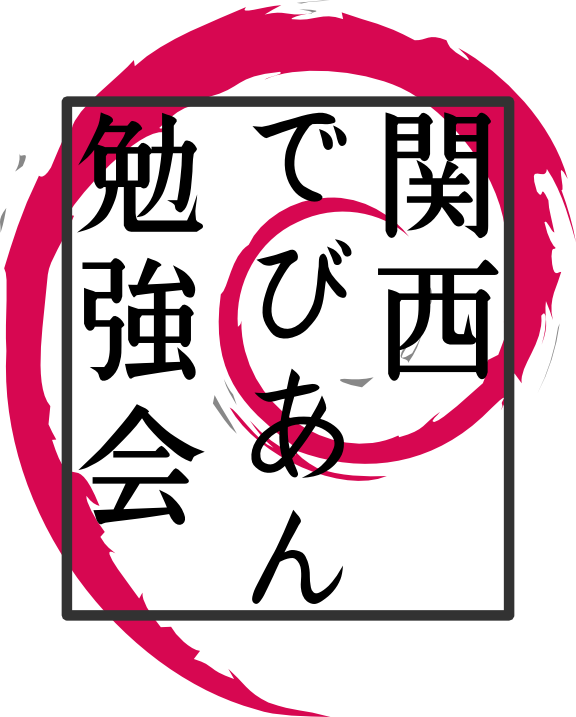
\includegraphics{image200802/kansaidebianlogo.png}
\end{center}

\begin{flushright}
\hfill{}関西 Debian 勉強会担当者 佐々木・倉敷・のがた \\
\hfill{}\debmtgyear{}年\debmtgmonth{}月\debmtgdate{}日
\end{flushright}

\thispagestyle{empty}
\end{titlepage}

\dancersection{Introduction}{Debian JP}

\subsection*{}%ロゴ用のスペース稼ぎ

関西 Debian 勉強会は Debian GNU/Linux のさまざまなトピック (新しいパッケー
ジ, Debian 特有の機能の仕組, Debian 界隈で起こった出来事, などなど) に
ついて話し合う会です.

目的として次の三つを考えています.
\begin{itemize}
      \item ML や掲示板ではなく, 直接顔を合わせる事での情報交換の促進
      \item 定期的に集まれる場所
      \item 資料の作成
\end{itemize}

それでは, 楽しい一時をお楽しみ下さい.

\clearpage

\begin{minipage}[b]{0.2\hsize}
 {\rotatebox{90}{\fontsize{80}{80}
{\gt 関西 Debian 勉強会}}}
\end{minipage}
\begin{minipage}[b]{0.8\hsize}
\hrule
\vspace{2mm}
\hrule
\setcounter{tocdepth}{1}
\tableofcontents
\vspace{2mm}
\hrule
\end{minipage}


\dancersection{最近の Debian 関係のイベント報告}{Debian JP}

\subsection{第 50 回関西 Debian 勉強会}
50 回目の関西 Debian 勉強会は 2011 年 8 月 28 日(日)に京都で開催されました。

いつもと違った雰囲気のよい会場でしたね、また利用させて頂きたい会場です。

\subsection{第 80 回東京エリア Debian 勉強会}
9 月の東京エリア Debian 勉強会は通常の勉強会ではなく 2011 年 9 月 17 日(土)、
18 日(日) の二日間に渡っての温泉合宿でした。

黙黙と開発をするストイックな開発合宿だったようです。

\clearpage
%-------------------------------------------------------------------------------
\dancersection{事前課題}{Debian JP}

今回は以下の事前課題を設定しました。


\begin{enumerate}
\item Debian パッケージの作成手順を復習しておいてください。先月(2011年08月)の勉強会資料が参考になるでしょう。
\item {bzr,git}-buildpackage パッケージがインストールされた環境を用意しておいてください。
\end{enumerate}

参加者の皆さんによる回答は以下の通りです。


\begin{prework}{ 山下尊也 }
(無回答)
\end{prework}

\begin{prework}{ Takuspeed83 }
(無回答)
\end{prework}

\begin{prework}{ Y.YATSUO }
(無回答)
\end{prework}

\begin{prework}{ 木下 }
\begin{enumerate}
\item ここしばらく立て込んでいまして・・・\\
すみません。時間取れていません。
\item 遅いノートですが入れときます。\\
自宅マシンにログインしようかな・・・
\end{enumerate}
\end{prework}

\begin{prework}{  清野陽一 }
(無回答)
\end{prework}

\begin{prework}{ 山田 洋平 }
\begin{enumerate}
\item 勉強しておきます。先月は出来たので、大丈夫な、はず。
\item 完了。あ、最初 sid 環境に chroot するの忘れて親環境にインストールしてました...
\end{enumerate}
\end{prework}

\begin{prework}{ kozo2 }
\begin{enumerate}
\item 先月の勉強会資料をやり直すことで復習しました。
\item 以下VirtualBoxゲストOSsidの端末出力です。
\begin{commandline}
root@debian:~# lsb_release -a |grep Description
No LSB modules are available.
Description:	Debian GNU/Linux unstable (sid)
root@debian:~# aptitude show bzr-buildpackage
No current or candidate version found for bzr-buildpackage
Package: bzr-buildpackage
State: not a real package
Provided by: bzr-builddeb
root@debian:~# aptitude show bzr-builddeb git-buildpackage |egrep 'Package|State'
Package: bzr-builddeb
State: installed
Package: git-buildpackage
State: installed
\end{commandline}
\end{enumerate}
\end{prework}

\begin{prework}{ yabuki@netfort.gr.jp }
ちょっと、遅くなるかも知れませんが行きますので。
\end{prework}

\begin{prework}{ かわだてつたろう }
資料読み直して用意しておきます。
\end{prework}

\begin{prework}{ 川江 }
\begin{enumerate}
\item これはしときます。
\item できるかな?
\end{enumerate}
\end{prework}

\begin{prework}{ 佐々木洋平 }
というわけで、先々月(?) の git-buildpackage 編のおさらいから始めてみます。
\end{prework}

\begin{prework}{ よしだともひろ }
\begin{enumerate}
\item 先月頂いた資料読んでおきます。
\item bzr-buildpackageとgit-buildpackageは入れました。
\end{enumerate}
\end{prework}



\clearpage
%------------------------------------------------------------------------------
\dancersection{vcs-buildpackage $\sim$bzrの場合$\sim$}{山下尊也}

\subsection{はじめに}

あなたは、vcs を使っていますか?
分散型バージョン管理システムが注目されるようになった頃から、
Linuxカーネルなどでも用いられており、開発スピードの早いGitを使っている方
が多い気がします。
はてなブックマーク\footnote{\url{http://b.hatena.ne.jp/}}などを見ていて
も、上位の記事になるのはGitばかりで、Bazaar使いとしてはとても悲しくなります。

私は、日々様々なファイルを扱っていますが、それらは Bazaar(bzr:バザー) を
使って管理しています\footnote{Bazaarを用いるようになった理由は、ファイル名が
Unicode 文字列で管理されていたからです。}。
そのためか、パッケージもBazaarを用いて管理していましたが、
最初のうちは適当に自分のリポジトリを作成し管理していました。
無理やりパッケージの管理をしていたため、他の手法を探していると、
bzr-builddeb があったので、それ以来bzr-builddebを使って管理しています。

\subsection{bzr-builddebの基本}

まずは、パッケージのインストールをしてみましょう。

\begin{commandline}
 $ sudo aptitude update
 $ sudo aptitude install bzr-builddeb
\end{commandline}

lenny では 0.95、squeeze では 2.4.2、sid では 2.7.8がインストール
されます。

\begin{commandline}
 $ dpkg -L bzr-builddeb  | grep bin
/usr/bin
/usr/bin/bzr-buildpackage
 $ bzr-buildpackage --help
Purpose: Builds a Debian package from a branch.
Usage:   bzr builddeb [BRANCH_OR_BUILD_OPTIONS...]

Options:
...[snip]
\end{commandline}

ヘルプに書かれている通り、ブランチからDebianパッケージを生成することを目
的としたコマンドです。


\begin{commandline}
 $ bzr help commands
[snip] 一部抜粋
bd-do             Run a command in an exported package, copying the result
                  back. [builddeb]

builddeb          Builds a Debian package from a branch. [builddeb]
Aliases: bd

dep3-patch        Format the changes in a branch as a DEP-3 patch. [builddeb]

dh-make           Helps you create a new package. [builddeb]
Aliases: dh_make

import-dsc        Import a series of source packages. [builddeb]

import-upstream   Imports an upstream tarball. [builddeb]

mark-uploaded     Mark that this branch has been uploaded, prior to pushing it.
                  [builddeb]

merge-package     Merges source packaging branch into target packaging branch.
                  [builddeb]

merge-upstream    Merges a new upstream version into the current branch.
                  [builddeb]
Aliases: mu
\end{commandline}

\verb|bzr|は他のVCSを使ったことがある人であれば、一通り使えると思います。
\verb|bzr help commands|でコマンドの一覧を見ることができるので、
分からないときは活用してください。
一覧の中で\verb|[builddeb]|がbzr-buildpackagで追加されたコマンドです。

\subsection{bzr-builddebで選択できるモード}

bzr-builddebでは、さまざまなモードがあらかじめ用意されています。
パッケージのメンテナが使いたいスタイルに応じて、モードを選択することがで
きます。
\fgref{bzr-select-mode}に示すのは、メンテナのスタイルに応じた
モードの選択肢です。

\begin{description}
 \item[Q1] 管理したいパッケージは
	    native package\footnote{Debian固有のパッケージ。また
	    は、ローカルでの使用のためだけに、メンテナンスしているソース
	    ファイルを含むパッケージ。例えば、debootstrapや
	    debian-el,debian-archive-keyringなど}ですか?
 \item[Q2] あなたがアップストリームメンテナーか?
 \item[Q3] debian/ ディレクトリ以下だけを保管したいのか?
 \item[Q4] パッケージ作業するときに、ブランチを分けて作業したいか?
\end{description}

\begin{figure}[h]
 \begin{center}
  \includegraphics[width=0.6\hsize]{image201109/bzr-builddeb-selectmode.eps}
 \end{center}
 \caption{bzr-builddebでのモードの選択}
 \label{bzr-select-mode}
\end{figure}

\clearpage

\subsection{Normal modeを用いたパッケージの管理}

\subsubsection{新規にパッケージを作る場合}

bzr-builddeb を用いて、パッケージを新規で作成する際は、
\verb|bzr dh-make|を用います\footnote{マニュアルには、開発段階の
ため別の場所でdh-makeして、debianディレクトリのファイルをコピーしろと
書かれていますが、bzr dh-makeで大丈夫でしょう。}。

\begin{commandline}
 $ mkdir ~/src-debian-normal
 $ bzr init-repo auto-install-el
 $ cd auto-install-el
 $ bzr init unstable
 $ cd unstable

 $ bzr dh-make auto-install-el 1.53 ../auto-install-el_1.53.orig.tar.gz
Fetching tarball
Looking for a way to retrieve the upstream tarball
Upstream tarball already exists in build directory, using that
Committing to: /tmp/test/auto-install-el/unstable/
added auto-install.el
Committed revision 1.

Type of package: single binary, indep binary, multiple binary, library,
 kernel module, kernel patch?
 [s/i/m/l/k/n] s

Maintainer name  : Takaya Yamashita
Email-Address    : takaya@debian.or.jp
Date             : Sun, 25 Sep 2011 01:01:31 +0900
Package Name     : auto-install-el
Version          : 1.53
License          : blank
Type of Package  : Single
Hit <enter> to confirm:
Skipping creating ../auto-install-el_1.53.orig.tar.gz because it already
 exists
Currently there is no top level Makefile. This may require additional
 tuning.
Done. Please edit the files in the debian/ subdirectory now. You should
 also
check that the auto-install-el Makefiles install into $DESTDIR and not
 in / .
Package prepared in /tmp/test/auto-install-el/unstable
 $ ls
auto-install.el  debian/
\end{commandline}

\begin{commandline}
 $ ls -1 debian
README.Debian
README.source
auto-install-el.cron.d.ex
auto-install-el.default.ex
auto-install-el.doc-base.EX
changelog
compat
control
copyright
docs
emacsen-install.ex
emacsen-remove.ex
emacsen-startup.ex
init.d.ex
manpage.1.ex
manpage.sgml.ex
manpage.xml.ex
menu.ex
postinst.ex
postrm.ex
preinst.ex
prerm.ex
rules*
source/
watch.ex

 $ bzr status
added:
  debian/
  debian/README.Debian
  debian/README.source
  debian/changelog
  debian/compat
  debian/control
  debian/copyright
  debian/docs
  debian/rules
  debian/source/
unknown:
  debian/auto-install-el.cron.d.ex
  debian/auto-install-el.default.ex
  debian/auto-install-el.doc-base.EX
  debian/emacsen-install.ex
  debian/emacsen-remove.ex
  debian/emacsen-startup.ex
  debian/init.d.ex
  debian/manpage.1.ex
  debian/manpage.sgml.ex
  debian/manpage.xml.ex
  debian/menu.ex
  debian/postinst.ex
  debian/postrm.ex
  debian/preinst.ex
  debian/prerm.ex
  debian/watch.ex
  debian/source/format

 $ bzr log -v --include-merges
------------------------------------------------------------
revno: 1
tags: upstream-1.53
committer: Takaya Yamashita <yamashita@takaya.biz>
branch nick: unstable
timestamp: Sun 2011-09-25 01:01:30 +0900
message:  Import upstream version 1.53
added:  auto-install.el

 $ edit
 $ edit
 $ edit
[snip]
 $ bzr builddeb
\end{commandline}

\subsubsection{既存のパッケージを bzr-builddeb で管理する場合}

\begin{commandline}
 $ mkdir ~/src-debian-normal
 $ bzr init-repo auto-install-el
 $ cd auto-install-el

 $ apt-get source auto-install-el

 $ bzr init unstable
 $ cd unstable
 $ bzr import-dsc ../*.dsc
Committing to: /home/takaya/src-debian-normal/auto-install-el/tmpriXU3G/upstream/
added auto-install.el
Committed revision 1.
All changes applied successfully.
Committing to: /home/takaya/src-debian-normal/auto-install-el/unstable/
added .pc
added debian
added .pc/.quilt_patches
added .pc/.quilt_series
added .pc/.version
added debian/README.Debian
added debian/changelog
added debian/compat
added debian/control
added debian/copyright
added debian/dirs
added debian/emacsen-install
added debian/emacsen-remove
added debian/emacsen-startup
added debian/rules
added debian/source
added debian/source/format
Committed revision 2.

 $ bzr log -v --include-merges
------------------------------------------------------------
revno: 2
tags: 1.48-1
fixes bug(s): http://bugs.debian.org/586177
author: Takaya Yamashita <takaya@debian.or.jp>
committer: Takaya Yamashita <yamashita@takaya.biz>
branch nick: unstable
timestamp: Tue 2010-06-15 23:16:42 +0900
message:
  Initial release (Closes: #586177)
added:
  .pc/
  .pc/.quilt_patches
  .pc/.quilt_series
  .pc/.version
  debian/
  debian/README.Debian
  debian/changelog
  debian/compat
  debian/control
  debian/copyright
  debian/dirs
  debian/emacsen-install
  debian/emacsen-remove
  debian/emacsen-startup
  debian/rules
  debian/source/
  debian/source/format
------------------------------------------------------------
revno: 1
tags: upstream-1.48
author: Takaya Yamashita <takaya@debian.or.jp>
committer: Takaya Yamashita <yamashita@takaya.biz>
branch nick: upstream
timestamp: Tue 2010-06-15 23:16:42 +0900
message:
  Import upstream version 1.48
added:
  auto-install.el

 $ bzr merge-upstream ../auto-install-el-1.53.orig.tar.gz --version 1.53
 --distribution debian --package auto-install-el
下記でも大丈夫
 $ bzr merge-upstream ../auto-install-el_1.53.orig.tar.gz --version 1.53
Using distribution unstable
Using version string 1.53.
Committing to: /home/takaya/src-debian-normal/auto-install-el/tmpNlFI08/upstream/
modified auto-install.el
Committed revision 2.
All changes applied successfully.
The new upstream version has been imported.
You should now review the changes and then commit.
\end{commandline}

\verb|bzr merge-upstream| コマンドを用いて、アップストリームの
ソースファイルをインポートします。
拡張子では \verb|.tar.gz, .tar, .tar.bz2, .tar.lzma, .tgz, .zip|に
対応しています\footnote{LZMA/XZ/Lzip の対応については、Bug 499484に
wishlist として報告されています。これらについては、アップストリームの
trunk では改善しているようです}。

また、ワーキングツリーの変更を行わずにアップストリームの変更をインポート
する\verb|bzr import-upstream|もあります。

\subsection{Merge modeを用いたパッケージの管理}

Merge modeはNormal modeに比べて少し複雑な作業が必要になってきます。
コマンドなども整備されていませんが、debianディレクトリ以下だけを
リポジトリに管理することができる利点があります。
また、共同で作業するときなどは、ファイルサイズを抑えることができます。

\begin{commandline}
 $ mkdir ~/src-debian/
 $ bzr init-repo ~/src-debian/twittering-mode
 $ cd ~/src-debian/twittering-mode
 $ bzr init unstable
 $ cd unstable
 $ mkdir .bzr-builddeb/
 $ echo -e '[BUILDDEB]\nmerge = True' > .bzr-builddeb/default.conf
 $ bzr add .bzr-builddeb/default.conf
\end{commandline}

本来、アップストリームから新しいバージョンが出た際は、\verb|bzr merge-upstream|を用います
が、Merge mode では対応していないため\footnote{changelog に対象とした
リリースを反映させることができない? bzr merge-upstream で --distribution
を使えばいけるかも-}、
バージョン番号を指定してあげる必要があります。
\footnote{debianディレクトリを別の場所で管理しているため、Bazaarの履歴が
受け継がれません。}

\begin{commandline}
 $ dch -v 2.0.0+git20110905-1
[snip]
 $ bzr builddeb
 $ ../dput debexpo twittering-mode_2.0.0+git20110905-1_amd64.changes
 $ bzr ci -m "New upstream version 2.0.0+git20110905"
\end{commandline}

処理を見ると、
\verb&~/src-debian/twittering-mode/build-area&
にて \verb|debuild| の作業が行われています。

また、backports向けにパッケージを作る際は、backports専用のbranchを
作成して、そこで作業しています。

\begin{commandline}
 $ cd ~/src-debian/twittering-mode
 $ bzr branch unstable bpo
 $ cd bpo
 $ bzr bd-do "dch --bpo"
[snip]
 $ bzr builddeb
[snip]
 $ ls -1 ../*bpo*
../auto-install-el_1.53-1~bpo60+1.debian.tar.gz
../auto-install-el_1.53-1~bpo60+1.dsc
../auto-install-el_1.53-1~bpo60+1_all.deb
../auto-install-el_1.53-1~bpo60+1_amd64.build
../auto-install-el_1.53-1~bpo60+1_amd64.changes
\end{commandline}

既存のパッケージをMerge modeに移行する場合は、
リポジトリを作成し、debianディレクトリをコピーすれば良いでしょう。

\begin{commandline}
 $ mkdir ~/src-debian/
 $ bzr init-repo ~/src-debian/twittering-mode
 $ cd ~/src-debian/twittering-mode

 $ apt-get source twittering-mode

 $ bzr init unstable

 $ cp -r twittering-mode-2.0.0+git20110905/debian ~/src-debian/twittering-mode/unstable

 $ cd unstable
 $ mkdir .bzr-builddeb/
 $ echo -e '[BUILDDEB]\nmerge = True' > .bzr-builddeb/default.conf
 $ bzr add .bzr-builddeb/default.conf

 $ bzr add .
 $ bzr ci -m "initial commit"
 $ bzr builddeb
\end{commandline}


\verb|bzr bd-do|を使うと、build-area
に一時的にコピーを行い、\verb|dpatch| などのコマンドを使用することができ
るようです\footnote{未検証}。

\subsection{管理していく上でのヒント}

普段はGPG署名をせずに、必要なときだけパッケージに署名を行なっている人も
多いと思います。
\verb|--|の後にコマンドを足すことによって、builderにオプションを渡すこと
ができます。

\begin{commandline}
 $ debuild -rfakeroot -us -uc
 $ bzr bd -- -us -uc
\end{commandline}
%$
\clearpage
%------------------------------------------------------------------------------
\dancersection{vcs-buildpackage $\sim$Gitの場合(again)$\sim$}{佐々木洋平さん}



\subsection*{はじめに}
\label{sec-1}
\subsubsection*{話の枕}
\label{sec-1-1}


山下さんの bzr 編に引い続き、
ここでは佐々木が Git を用いて
Debian パッケージを作成する場合についてまとめます。
前々回(2011年06月, 第48回)でも \texttt{git-buildpackage}
について(簡単に)触れましたが、
その後ちゃんと調べたら、幾つかコマンドが新しく追加されていたりしました。
ですので、前々回の復習も兼ねて
「Git を使って Debian パッケージを作成/管理するお話」をしてみたいと思います。
\subsubsection*{前提とする知識と目的}
\label{sec-1-2}


とはいえ、パッケージング全てについて触れる事はできませんので、ここでは
\begin{itemize}
\item source package についてのある程度の知識
\item Git に関して, 特に tag と branch についてのある程度の知識
\end{itemize}
があることを前提としています。
最後に参考文献していますので、
適宜参照して下さい、もしくは質問して下さい。

\subsubsection*{パッケージ作成作業(復習)}
\label{sec-1-3}

通常、パッケージ作成は

\begin{enumerate}
\item upstream のソースを取得
\item (場合によっては) non-free な部分を除いたりして、
\item \texttt{./debian} ディレクトリ以下を作成/更新して、
\item 場合によっては upstream のソースにパッチを当てて、
\item ソース/バイナリ パッケージをビルド
\end{enumerate}

という事を行ないます。これらの作業を VCS で管理します。

\subsubsection*{典型的なリポジトリレイアウト}
\label{sec-1-4}

前回お話した \texttt{git-import-dsc} で
既存のソースパッケージを import したり、
\texttt{debcheckout} で Git で管理されているパッケージを
checkout すると、
多くの場合、リポジトリは以下の様になります。
\begin{commandline}
  $ git branch
  * master             <-- debian/ 入りのフルソース
    pristine-tar       <-- orig.tar.{gz,bz2} のバイナリデルタ
    upstream           <-- debian/ 無し(upstream)のソース
\end{commandline}
%$
ここで \texttt{git-buildpackage} を実行すると、
パッケージのビルドが始まります。
今日は\textbf{この状態に持って行くまで}の話にフォーカスしてみます。

\subsection*{upstream ソースを import するには?}
\label{sec-2}
\subsubsection*{upstream ソースを import するには?}
\label{sec-2-1}

upstream のソースを持ってきて、
Git リポジトリを作成することを考えると、
\begin{itemize}
\item simple な場合
  \begin{enumerate}
  \item tarball を展開して import
  \item upstream の VCS を import
  \end{enumerate}
\item 調整が必要な場合
  \begin{itemize}
  \item non-dfsg-free な部分を削除してから import
  \end{itemize}
\end{itemize}
...でしょうか?

注意すべきは \texttt{pristiner-tar} を用いること、です。

\subsubsection*{pristine-tar ?}
\label{sec-2-2}

gzip の圧縮率の違いなどから、
\texttt{upstream}ブランチから生成された .tar.gz は upstream の配布物と異なる事があります。
\texttt{pristine-tar} によって、
upstream の tarball を import する際にバイナリデルタを保存しておくことで、
\texttt{upstream} ブランチから tarball(\texttt{.orig.tar.gz}) を生成する際に、
checksum の等しい tarball を生成することができます。

このバイナリデルタは \texttt{pristine-tar} ブランチに保存されます。
もし忘れた場合には
\begin{commandline}
  $ pristine-tar commit foobar.tar.gz [upstream の tag]
  $ pristine-tar checkout ../foobar.tar.gz
\end{commandline}
の様にして後からコミットできますが、
最初に import する際に忘れずにバイナリデルタを保存しておくのが良いでしょう。
\texttt{git-import-orig} コマンドにはオプションとして \texttt{--pristine-tar}があります。
ごく稀に上手くバイナリデルタを生成できない tarball がある(らしい)ですが...

\subsubsection*{upstream の VCS から import する}
\label{sec-2-3}

注意すべきは \textbf{tarballも必ず import すること} でしょうか?
これは、履歴とともにバイナリデルタを保持するために必要な作業です。

また、リリースされている tarball は Tag が打たれている(もしくはそれに類するコミットがある)ハズなので、
履歴を適宜修正すると upstream のコミットを patch として管理しやすくなります。

\subsubsection*{upstream の VCS から import する(1)}
\label{sec-2-4}

幸運にも upstream が Git だったら

\begin{commandline}
$ git remote add upstream-repos [url]
$ git fetch upstream-repos
$ git co upstream && git merge upstream-repos
\end{commandline}
%$
で ok です。

\subsubsection*{upstream の VCS から import する(2)}
\label{sec-2-5}

Subversion の場合は \texttt{git-svn} を用います。
毎度 rebase しながら作業することになるので、大変面倒ですが...%
\footnote{もっと良い方法ありませんかね?}

\begin{itemize}
\item Subversion: 初回
\end{itemize}
\begin{commandline}
$ git-svn init [url]
$ git svn fetch
$ git log ref/remotes/git-svn
$ git checkout -b upstream refs/remotes/git-svn
$ git push origin upstream:upstream
\end{commandline}
%$
\begin{itemize}
\item Subversion: 二回目以降
\end{itemize}
\begin{commandline}
$ git config --remove-section svn-remote.svn 1>/dev/null 2>&1
$ git svn init [url]
$ git show-ref origin/upstream > \
   `git rev-parse-git-dir`/refs/remotes/git-svn
\end{commandline}
%$

\subsubsection*{tarball を import するツール}

以下では, tarball を import するコマンド群についてまとめておきます。

\label{sec-2-6}
\paragraph{\texttt{git-import-orig}}
\label{sec-2-6-1}
\begin{itemize}
\item \texttt{git-buildpackage} パッケージで提供
  \begin{itemize}
  \item simple に tarball を import
  \item (Optionつければ) pristine-tar も実行
  \item (あれば)現状の master ブランチへ自動で merge して
  \item タグも打ってくれる
  \end{itemize}
\item 一番 simple
  \begin{itemize}
  \item 必要な事は全てやってくれるので, これで十分な事が多い。
  \end{itemize}
\end{itemize}
\label{sec-2-6-2}

\label{sec-2-7}
\paragraph{\texttt{git-dpm import-new-upstream}}
\label{sec-2-7-1}

\begin{itemize}
\item \texttt{git-dpm}: git Debian package manager
\item 動作は git-import-orig とほぼ同じ
\item VCS の履歴との対応や \texttt{patch-queue}ブランチ(後述)の生成/管理もしてくれる
\end{itemize}

\subsubsection*{調整が必要な場合(1)}
\label{sec-2-8}

upstream の配布物に non-dfsg-free な部分があったりして調整が必要な場合は
\begin{itemize}
\item upstream ブランチで non-dfsg-free な部分を削除/調整
\item new upstream version として merge/commit
\item tarball として repack した後に import/タグ打ち
\end{itemize}
なんて事をします。例えば

\begin{commandline}
$ git checkout upstream
$ git merge -s recursive -X theirs [upstream tag]
\end{commandline}

もしくは

\begin{commandline}
$ git status -s | egrep '^(DU|UA| U|UD)' | cut -c4- | \
    xargs git rm --ignore-unmatch DUMMY$$
$ git commit
\end{commandline}

とか?

uscan に repack 用の hook script を使っているなら、それを実行したのち
tarball として import する、の方が楽かもしれません。


\subsection*{\texttt{./debian} をガシガシ書く/修正する}
\label{sec-3}

まあこれは良いですよね?
\begin{commandline}
  $ git branch
  * master
    pristine-tar
    upstream
\end{commandline}
%$

\begin{itemize}
\item upstream のソースは全て Git リポジトリの\texttt{upstream} ブランチ
\item \texttt{./debian} での変更は \texttt{master} ブランチで
  \begin{itemize}
  \item 全ての変更は \texttt{master} 内で行なう
  \item 何をしたのかは \texttt{git log} で容易に追跡できる
  \item patch も作成しやすい
  \end{itemize}
\end{itemize}
となります。Happy Hacking!!

\subsection*{patch を扱うには?}

source format 3.0 (quilt) では、
upstream への変更点を {\tt{quilt}} を用いてパッチで管理します。

\label{sec-4}
\subsubsection*{単純な方法}
\label{sec-4-1}

Git の事は忘れて quilt だけでパッチを作成
(もしくは debuild が走った際にパッチとして抽出)する、です。

複雑な事は何もありませんが、VCS の恩恵を受けることもありません。

\subsubsection*{git を使う場合(1)}
\label{sec-4-2}

逆に quilt を忘れて Git だけで patch を管理する方法です。
debuild 等で patch を生成し, {./debian/patches/} 以下を
git で管理します。
%
まあ VCS っぽく管理するなら
1 パッチ/1コミットとして手動で管理するのでしょうか?
%
\subsubsection*{patch ブランチで}
\label{sec-4-3}

パッチ\textbf{だけ}を track するための branch を用意して、
1パッチ/1ブランチ or 1パッチ/1コミットとして管理します。
注意すべきは
\begin{itemize}
\item quilt への export を行なうには
  コミット履歴が\textbf{綺麗}でないといけない
  \begin{itemize}
  \item 1 パッチ/1コミット
  \item squash !! squash !! squash !!
  \end{itemize}
\item 今のところ 1-way rebase なので、upstream の更新をする度に
  作業が必要。
\end{itemize}

以下, 幾つかのコマンドについて述べます。

\label{sec-4-5}
\paragraph{topgit: a Git patch queue manager}
\label{sec-4-5-1}

\begin{itemize}
\item コミット履歴をブランチで管理
\item パッチ間の依存関係も管理
\item 便利だけど, やりすぎな気もしないでもない
\item \texttt{patch-queue} ブランチから quilt へ export したパッチは
  \texttt{master} ブランチにコミットしておく必要がある
\end{itemize}

\paragraph{gbp-pq}
\label{sec-4-7-1}

\begin{itemize}
\item \texttt{git-buildpackage} で提供
\item \texttt{git format-patch} の wrapper
\item 1パッチ/1コミット, として patch を生成/取り込み
\item \texttt{master} を rebase して使う
\end{itemize}
\label{sec-4-7-2}
\begin{commandline}
$ git checkout master ; git branch -D patch-queue
$ quilt pop -a
$ gbp-pq import
 ... 作業 ...
$ git checkout master ; gbp-pq export
\end{commandline}

\paragraph{git-dpm}
\label{sec-4-8-1}

\begin{itemize}
\item パッチは一つのブランチで管理
\item 1パッチ/1コミット
\item パッチは \texttt{master} ブランチに merge されたままで管理
\item パッチが当たった \texttt{upstream} ブランチを rebase
\item プライベートブランチの SHA1 ハッシュを
      \texttt{./debian/.git-dpm} に保存
\end{itemize}
\label{sec-4-9}
\paragraph{gitpkg の quilt export hook}
\label{sec-4-9-1}

\begin{itemize}
\item 1パッチ/1コミット, などという制限は無い
\item \texttt{debian/source/git-patches} に設定を書く
\end{itemize}
    \begin{commandline}
    upstream/[UPSTREAM_REF]...patche-queue1/[DEBIAN_REF1]
    upstream/[UPSTREAM_REF2]...topic1/[DEBIAN_REF2]
    \end{commandline}
\begin{itemize}
\item パッチはコミットされない
\item tag は再生成される
\end{itemize}

\subsection*{source package の生成}
\label{sec-5}

\label{sec-5-1}
\paragraph{git-dpm}
\label{sec-5-1-1}

\begin{itemize}
\item ビルド用の特定のコマンドは無い(\texttt{dpkg-source -b} とか)
\end{itemize}
\paragraph{gitpkg}
\label{sec-5-1-2}

\begin{itemize}
\item pristine-tar, \texttt{upstream} ブランチから tarball を生成し
      source package をビルド
\end{itemize}
\paragraph{git-buildpackage}
\label{sec-5-1-3}

\begin{itemize}
\item default. バイナリパッケージも作成する
\item \texttt{git-pbuilder}: pbuilder/cowbuilder を呼び出せる
\item タグを打ったり.
\end{itemize}
\subsection*{まとめ(?)}
\label{sec-6}

いろいろコマンドが増えてきましたが、結局のところ
\texttt{git-buildpackage} が一番簡単/便利/移行コストも低い、
という印象です。workflow が他の vcs-buildpackage と似ているから、
でしょうか。

また git-dpm/gitpkg は
workflow/patch-queue の自由度は高い(けれど, 複雑になりがち)、
な印象を受けます。

git-dpm パッケージは提供するコマンドが多くて、
\begin{itemize}
  \item コマンドが多くて, ちょっと敷居が高い(かも)
  \item 一番「git らしく」作業できる(らしい)
\end{itemize}
ですね。また、
\begin{itemize}
\item gitpkg
  \begin{itemize}
  \item hook での拡張/カスタマイズが容易.
  \item リポジトリのレイアウトも固定されていない
  \end{itemize}
\end{itemize}
です。


\clearpage
%-------------------------------------------------------------------------------
\dancersection{今後の予定}{Debian JP}

\subsection{第52回関西 Debian 勉強会}

第 52 回関西 Debian 勉強会は、10 月 23 日(日)に福島区民センターで開催する予定です。
発表内容については未定ですので、みなさまの発表をお待ちしております。

\subsection{第53回関西 Debian 勉強会 in KOF 2011 }

11 月の関西 Debian 勉強会は、11 月 12 日(土)の関西オープンソース 2011 において
セッションとして開催します。

「Debian Updates」という毎度タマムシ色のお題で話者は佐々木の予定です。

% 冊子にするために, 4 の倍数にする必要がある.
% そのための調整
\dancersection{メモ}{}
\mbox{}\newpage
\mbox{}\newpage
\mbox{}\newpage

\printindex
% \cleartooddpage

 \begin{minipage}[b]{0.2\hsize}
  \rotatebox{90}{\fontsize{80}{80} {\gt 関西 Debian 勉強会} }
 \end{minipage}
 \begin{minipage}[b]{0.8\hsize}

 \vspace*{15cm}
 \rule{\hsize}{1mm}
 \vspace{2mm}
 
\includegraphics[width=2cm]{image200502/openlogo-nd.eps}
 \noindent \Large \bf Debian 勉強会資料\\ \\
 \noindent \normalfont \debmtgyear{}年\debmtgmonth{}月\debmtgdate{}日 \hspace{5mm}  初版第 1 刷発行\\
 \noindent \normalfont 関西 Debian 勉強会 (編集・印刷・発行)\\
 \rule{\hsize}{1mm}
 \end{minipage}

\end{document}
